\documentclass{sigplanconf}

\usepackage{epsfig}
\usepackage{amsmath}
\usepackage{mathpartir}
\usepackage{graphicx}
\usepackage{boxedminipage}
\usepackage{latexsym}
\usepackage{balance}


\newcommand{\dataflow}{dataflow}
\newcommand{\dc}{\mbox{\sc DC}}
%\newcommand{\trans}{\,\Downarrow}
\newcommand{\trans}{\,\Rightarrow}
%\newcommand{\trans}{\, \rightarrow}
\newcommand{\normal}{\mbox{\tt{normal}}}
\newcommand{\reactive}{\mbox{\tt{reactive}}}
%\newcommand{\self}{\mbox{\tt{self}}}
\newcommand{\self}{\mbox{$c_{self}$}}
\newcommand{\pick}{\mbox{\tt{pick}}}
\newcommand{\newcons}{\mbox{\tt{newcons}}}
\newcommand{\delcons}{\mbox{\tt{delcons}}}
\newcommand{\while}{\mbox{\sc While}}
\newcommand{\dwhile}{\mbox{\sc DWhile}}
\newcommand{\wwhile}{\mbox{\bf while}}
\newcommand{\wdo}{\mbox{\bf do}}
\newcommand{\wskip}{\mbox{\bf skip}}
\newcommand{\wif}{\mbox{\bf if}}
\newcommand{\wthen}{\mbox{\bf then}}
\newcommand{\welse}{\mbox{\bf else}}
\newcommand{\emphasize}{\sc\small}
\newcommand{\sq}{\mbox{\sc sq}}
\newcommand{\csp}{\mbox{\sc csp}}
\newcommand{\grid}{\mbox{\sc Grid}}
\newcommand{\rgrid}{\mbox{\sc RGrid}}

\newtheorem{theorem}{Theorem}
\newtheorem{lemma}{Lemma}
\newtheorem{corollary}{Corollary}
\newtheorem{definition}{Definition}
\newtheorem{remark}{Remark}
\newtheorem{property}{Property}
\newtheorem{invariant}{Invariant}
\newtheorem{datastructure}{Data Structure}

\newenvironment{proof}
{\noindent   {\sc Proof.}}{\hspace*{\fill}$\Box$\par\vspace{2mm}}

\newenvironment{sketch}
{\noindent   {\sc Proof (sketch).}}{\hspace*{\fill}$\Box$\par\vspace{2mm}}

\newcommand{\fullpaper}[1]{}
\newcommand{\wmax}[1]{}
\newcommand{\consact}[1]{#1}
\newcommand{\colsp}{@{~~}}

%%%%%%%%%%%%%%%%%%%%%%%%%%%%%%%%%%%%%%%%%%%%%%%%%%%%%%%%%%%%%%%%%%%%%%%%%%%%%%
% ENVIRONMENT FOR PROGRAMS AND ALGORITHMS:  figprog
% REQUIRES TWO ARGUMENTS:                   label-string    caption
%
% EXAMPLE OF INVOCATION:
%
%       \begin{figprog}{alg:my-label}{My beautiful caption.}
%
%%%%%%%%%%%%%%%%%%%%%%%%%%%%%%%%%%%%%%%%%%%%%%%%%%%%%%%%%%%%%%%%%%%%%%%%%%%%%%

\newcommand{\LaBeL}{UNO}
\newcommand{\CaPtIoN}{DUE}
\newenvironment{figprog}[3]{%
\renewcommand{\LaBeL}{#1}%
\renewcommand{\CaPtIoN}{#2}%
\begin{figure}[#3]%
%\vspace{-.1in}%
\noindent~\hrulefill~%
\vspace{-.05in}%
\begin{prog}{\footnotesize}%
}{\end{prog}%
\vspace{-.10in}%
\noindent~\hrulefill~%
\vspace{-.08in}%
\caption{\CaPtIoN}%
\label{\LaBeL}%
\end{figure}%
}

\newcommand{\FoNtSiZe}{ONE}
\newenvironment{frameprog}[2]{%
\renewcommand{\FoNtSiZe}{#2}%
% \begin{center}%
\begin{minipage}{#1}%
% \vspace{10mm}%
% ~\hrulefill~%
% \vspace{-.05in}%
\begin{prog}{\FoNtSiZe}%
}{\end{prog}%
\vspace{-.10in}%
% ~\hrulefill~%
% \vspace{-.08in}%
\end{minipage}%
% \end{center}%
}



%%%%%%%%%%%%%
% Step numbering (within algorithms)

\newcounter{stepcount}
\newcommand{\steplabel}[1]{\newcounter{#1}\setcounter{#1}{\thestepcount}}
%%%%% Reference to step-labels:
%%%%% "\steplabel" must be before "\stepref"
\newcommand{\stepref}[1]{\arabic{#1}}

\newcounter{poi}
\newcommand{\N}{\stepcounter{poi} \< \thepoi . \>}
\newcommand{\RC}{\setcounter{poi}{0}}
\newcommand{\rem}[1]{\mbox{\rm \{#1\}}}
\newcommand{\rrem}[1]{\`\mbox{\rm\small \{#1\}}}
\newcommand{\srem}[1]{~~~~~\mbox{\rm \{#1\}}}
\newcommand{\linelabel}[1]{\newcounter{#1}\setcounter{#1}{\thepoi}}
\newcommand{\lineref}[1]{\arabic{#1}}
\newenvironment{prog}[1]{#1 %\tt%\small %%% eliminati \tt\small
\setcounter{poi}{0}
\vspace{-.15in}
\begin{tabbing}
=spa\=spa\=spa\=spa\=spa\=spa\=spa\=spa\=spa\=spa\=spa\=spa\=spa\=\kill
\+\\}{
\end{tabbing}
\vspace{-.15in}
}

%%%%%%%%%%%%%
% Commands: Programs and Pseudocode

\newcommand {\ALGORITHM}{\mbox{\bf algorithm}}
\newcommand {\AND}{\mbox{\bf and}}
\newcommand {\BEGIN}{\mbox{\bf begin}}
\newcommand {\BREAK}{\mbox{\bf break}}
\newcommand {\DO}{\mbox{\bf do}}
\newcommand {\CONTINUE}{\mbox{\bf continue}}
\newcommand {\EACH}{\mbox{\bf each}}
\newcommand {\ELSE}{\mbox{\bf else}}
\newcommand {\END}{\mbox{\bf end}}
\newcommand {\ENDWHILE}{\mbox{\bf endwhile}}
\newcommand {\ERROR}{\mbox{\bf ERROR}}
\newcommand {\EXIT}{\mbox{\bf EXIT}}
\newcommand {\FALSE}{\mbox{\bf false}}
\newcommand {\FOR}{\mbox{\bf for}}
\newcommand {\ENDFOR}{\mbox{\bf endfor}}
\newcommand {\FOREACH}{\mbox{\bf for each}}
\newcommand {\FUNCTION}{\mbox{\bf function}}
\newcommand {\IF}{\mbox{\bf if}}
\newcommand {\ENDIF}{\mbox{\bf endif}}
\newcommand {\GOTO}{\mbox{\bf goto}}
\newcommand {\HALT}{\mbox{\bf HALT}}
\newcommand {\LET}{\mbox{\bf let}}
\newcommand {\OR}{\mbox{\bf or}}
\newcommand {\NIL}{\mbox{\bf nil}}
\newcommand {\NOT}{\mbox{\bf not}}
\newcommand {\NULL}{\mbox{{\bf Null}}}
\newcommand {\PRINT}{\mbox{\bf print}}
\newcommand {\PROGRAM}{\mbox{\bf program}}
\newcommand {\PROCEDURE}{\mbox{\bf procedure}}
\newcommand {\REPEAT}{\mbox{\bf repeat}}
\newcommand {\REPORT}{\mbox{\bf report}}
\newcommand {\RETURN}{\mbox{\bf return}}
\newcommand {\STEP}{\mbox{\normalsize\bf Step}}
\newcommand {\THEN}{\mbox{\bf then}}
\newcommand {\TO}{\mbox{\bf to}}
\newcommand {\TRUE}{\mbox{\bf true}}
\newcommand {\UNTIL}{\mbox{\bf until}}
\newcommand {\WHILE}{\mbox{\bf while}}
\newcommand {\VAR}{\mbox{\bf var}}
\newcommand {\CASE}{\mbox{\bf case:}}
\newcommand {\ENDCASE}{\mbox{\bf endcase}}
\newcommand {\INPUT} {\mbox{\bf input}}
\newcommand {\OUTPUT} {\mbox{\bf output}}



\begin{document}

\conferenceinfo{PLDI'11,} {June 4--8, 2011, San Jose, California, USA.}
\CopyrightYear{2011}
\copyrightdata{978-1-4503-0663-8/11/06}

\title{Mining Hot Calling Contexts in Small Space}

 \authorinfo{Daniele Cono D'Elia}
            {Dept. of Computer and System Sciences\\Sapienza University of Rome}
            {danielecono.delia@gmail.com}
 \authorinfo{Camil Demetrescu}
            {Dept. of Computer and System Sciences\\Sapienza University of Rome}
            {demetres@dis.uniroma1.it}
 \authorinfo{Irene Finocchi}
            {Dept. of Computer Science\\Sapienza University of Rome}
            {finocchi@di.uniroma1.it}

\maketitle


\begin{abstract}
Calling context trees (CCTs) associate performance metrics with paths through a program's call graph, providing valuable information for program understanding and performance analysis. Although CCTs are typically much smaller than call trees, in real applications they might easily consist of tens of millions of distinct calling contexts: this sheer size makes them difficult to analyze and might hurt execution times due to poor access locality. For performance analysis, accurately collecting information about hot calling contexts may be more useful than constructing an entire CCT that includes millions of uninteresting paths. As we show for a variety of prominent Linux applications, the distribution of calling context frequencies is typically very skewed. In this paper we show how to exploit this property to reduce the CCT size considerably.

We introduce a novel run-time data structure, called {\em Hot Calling Context Tree (HCCT)}, that offers an additional intermediate point in the spectrum of data structures for representing interprocedural control flow. The HCCT is a subtree of the CCT that includes only hot nodes and their ancestors. We show how to compute the HCCT without storing the exact frequency of all calling contexts, by using fast and space-efficient algorithms for mining frequent items in data streams. With this approach, we can distinguish between hot and cold contexts on the fly, while obtaining very accurate frequency counts. We show both theoretically and experimentally that the HCCT achieves a similar precision as the CCT in a much smaller space, roughly proportional to the number of distinct hot contexts: this is typically several orders of magnitude smaller than the total number of calling contexts encountered during a program's execution. Our space-efficient approach can be effectively combined with previous context-sensitive profiling techniques, such as sampling and bursting.
\end{abstract}


\category{C.4}{Performance of Systems} {Measurement Techniques}
\category{D.2.2}{Software Engineering} {Tools and Techniques}[programmer workbench]
\category{D.2.5}{Software Engineering} {Testing and Debugging}[diagnostics, tracing]

\terms Algorithms, Measurement, Performance.

\keywords Performance profiling, dynamic program analysis, data streaming algorithms, frequent items, program instrumentation.


%--------------------------------------------------------------------------------
\section{Introduction}
\label{se:intro}

Context sensitive profiling provides valuable information for program understanding, performance analysis, and runtime optimizations. Previous works have demonstrated its effectiveness for tasks such as residual testing~\cite{PavlopoulouY99, VNC07}, function inlining~\cite{CMCH92}, statistical bug isolation~\cite{Feng03, Liblit03}, object allocation analysis~\cite{NethercoteS07}, or anomaly-based intrusion detection~\cite{BM07}. A {\em calling context} is a sequence of routine calls that are concurrently active on the run-time stack and that lead to a program location. Collecting context information in modern object-oriented software is very challenging: application functionalities are divided into a large number of small routines, and the high frequency of function calls and returns might result in considerable profiling overhead, Heisenberg effects, and huge amounts of contexts to be analyzed by the programmer.

Several data structures have long been used to maintain information about interprocedural control flow. In a {\em call graph}, nodes represent routines and arcs caller-callee relationships. The use of call graph profiles was pionereed by gprof~\cite{GKM82}, that attributes the time for each  routine to its callers by propagating times along edges of the call graph. Although very space- and time-efficient, this approach can lead to misleading results, as pointed out in~\cite{PF88, S04}. On the other side, each node of a {\em call tree} represents a different routine invocation. This yields very accurate context information, but requires extremely large (possibly unbounded) space.
The inaccuracy of call graphs and the huge size of call trees have motivated the introduction of {\em calling context trees (CCT)}~\cite{ABL97}: differently from call trees, CCTs do not distinguish between different invocations of the same routine within the same context. While maintaining good accuracy, typically CCTs are several orders of magnitude smaller than call trees: the number of nodes may be large in the presence of recursion, but this is seldom the case in practice. The exhaustive approach to constructing a CCT is based on the instrumentation of each routine call and return, incurring considerable slowdown even using efficient instrumentation mechanisms~\cite{ABL97,ZSCC06}. Sampled stack-walking reduces slowdown, but at the price of accuracy. The adaptive bursting mechanism proposed in~\cite{ZSCC06} selectively inhibits redundant profiling, dramatically reducing the overhead over the exhaustive approach while preserving good profile accuracy.

As noticed in previous works~\cite{BM07, ZSCC06}, even calling context trees may be very large and difficult to analyze in several applications. Moreover, their sheer size might hurt execution time due to poor access locality during construction and query. As an example, in Table~\ref{tab:CCTsize} we report the number of nodes of the call graph, call tree, and calling context tree for a variety of off-the-shelf applications in a typical Linux distribution. These numbers have been obtained from short runs of each application, which yield millions of calling contexts. The optimistic assumption that each CCT node requires 20 bytes (previous works use larger nodes~\cite{ABL97,S04}) already results in almost 1GB needed just to store a CCT with 48 million nodes for an application such as Open Office -- calc. To face this space issue, the approach proposed in~\cite{BM07} maintains a one-word probabilistically unique value per context, achieving minimal space overhead when all contexts have to be stored, but specific information about them is unnecessary. As noted in~\cite{BM07}, even this approach, however, can run out of memory on large traces with tens of millions of contexts.

\begin{table}[t]
\caption{Number of nodes of call graph, call tree, calling context tree, and number of distinct call sites for different applications.}
\centering
\begin{small}
\begin{tabular}{r r r r r}
\hline\hline
Application & $|$Call graph$|$ & Call sites & $|$CCT$|$ & $|$Call tree$|$\\
\hline
amarok & 13\,754 & 113\,362 & 13\,794\,470 & 991\,112\,563 \\
ark & 9\,933 & 76\,547 & 8\,171\,612 & 216\,881\,324 \\
audacity & 6\,895 & 79\,656 & 13\,131\,115 & 924\,534\,168 \\
bluefish & 5\,211 & 64\,239 & 7\,274\,132 & 248\,162\,281 \\
dolphin & 10\,744 & 84\,152 & 11\,667\,974 & 390\,134\,028 \\
firefox & 6\,756 & 145\,883 & 30\,294\,063 & 625\,133\,218 \\
gedit & 5\,063 & 57\,774 & 4\,183\,946 & 407\,906\,721 \\
ghex2 & 3\,816 & 39\,714 & 1\,868\,555 & 80\,988\,952 \\
gimp & 5\,146 & 93\,372 & 26\,107\,261 & 805\,947\,134 \\
gwenview & 11\,436 & 86\,609 & 9\,987\,922 & 494\,753\,038 \\
inkscape & 6\,454 & 89\,590 & 13\,896\,175 & 675\,915\,815 \\
oocalc & 30\,807 & 394\,913 & 48\,310\,585 & 551\,472\,065 \\
ooimpress & 16\,980 & 256\,848 & 43\,068\,214 & 730\,115\,446 \\
oowriter & 17\,012 & 253\,713 & 41\,395\,182 & 563\,763\,684 \\
pidgin & 7\,195 & 80\,028 & 10\,743\,073 & 404\,787\,763 \\
quanta & 13\,263 & 113\,850 & 27\,426\,654 & 602\,409\,403 \\
sudoku & 5\,340 & 49\,885 & 2\,794\,177 & 325\,944\,813 \\
vlc & 5\,692 & 47\,481 & 3\,295\,907 & 125\,436\,877 \\
\hline
\end{tabular}
\end{small}
\label{tab:CCTsize}
\end{table}

Although very useful, e.g., in bug or intrusion detection applications, probabilistic calling context was not designed for profiling with 
the purpose of understanding and improving application performance, where it is crucial to maintain for each context the sequence of active routine calls along with performance metrics. In this scenario, only the most frequent contexts are of interest, since they represent the hot spots to which optimizations must be directed. As observed in~\cite{ZSCC06}: ``Accurately collecting information about hot edges may be more useful than accurately constructing an entire CCT that includes rarely called paths.'' Figure~\ref{fig:skewness} shows that, for different applications, only a small fraction of contexts are hot: in accordance with the well-known Pareto principle, more than 90\% of routine calls take place in only 10\% of contexts. The skewness of context distribution suggests that space could be greatly reduced by keeping information about hot contexts only and discarding on the fly contexts that are likely to be cold, i.e., to have low frequency or to require small time throughout the entire execution. 

\paragraph{Our Contributions.} In this paper we introduce a novel run-time data structure, called {\em Hot Calling Context Tree (HCCT)}, that compactly represents all the hot calling contexts encountered during a program's execution, offering an additional intermediate point in the spectrum of data structures for representing interprocedural control flow. The HCCT is a subtree of the CCT that includes only hot nodes and their ancestors.
For each hot calling context, it also maintains an estimate of its performance metrics (for simplicity, we focus on frequency counts throughout the paper, but our approach can be easily extended to arbitrary metrics such as execution time, cache misses, or instruction stalls). Our main contributions can be summarized as follows:

\begin{itemize}

\item We formalize the concept of Hot Calling Context Tree and we cast the problem of identifying the most frequent contexts into a data streaming setting: we show that the HCCT can be computed without storing the exact frequency of all calling contexts, by using fast and space-efficient algorithms for mining frequent items in data streams. With this approach, we can distinguish between hot and cold contexts on the fly, while obtaining very accurate frequency counts. 

\item We implement three variants of space-efficient context-sensitive profilers based on three different streaming algorithms. For one of the algorithms, we devise  a highly tuned implementation that is more efficient in practice than the one proposed by the authors and that might be of independent interest.  

\item We integrate our space-efficient approach with previous techniques aimed at reducing time overhead: we focus in particular on static bursting and adaptive bursting with re-enablement~\cite{ZSCC06}, which offer very good time-accuracy tradeoffs.

\item We perform an extensive experimental analysis of performances and accuracy on a variety of prominent Linux applications. We test many different parameter settings and consider several metrics, including degree of overlap and hot edge coverage used in previous works.  The experiments not only confirm, but reinforce the theoretical prediction, showing that the HCCT represents the hot portions of the full CCT very well using only an extremely small percentage of the space required by the entire CCT. Even when the peak memory usage of our profilers is only $1\%$ of standard context-sensitive profilers, we can show the following:

\begin{itemize}
\item all the hottest calling contexts are always identified correctly (no false negatives);

\item frequency counters are very close to the true values;

\item the number of false positives (cold contexts that are considered as hot) is very small;

\item using bursting, the running time overhead can be kept under control without affecting accuracy in a substantial way. 
\end{itemize} 

\end{itemize}

\begin{figure}[t]
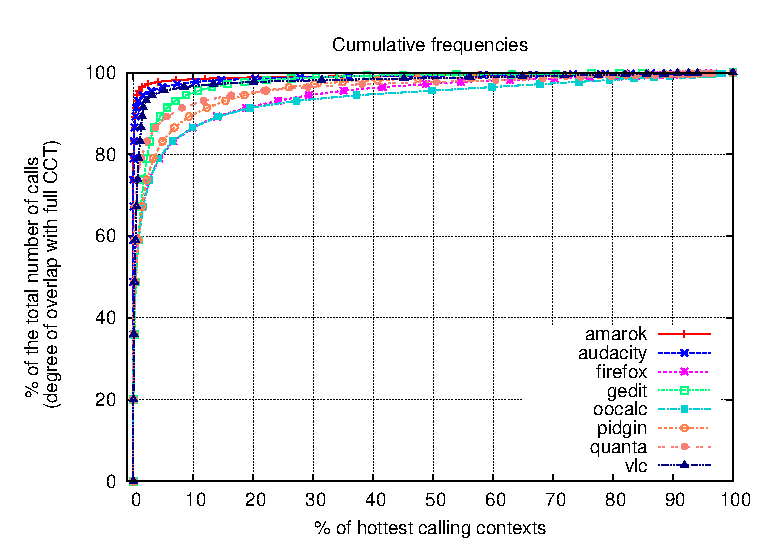
\includegraphics[width=\columnwidth]{charts/cumulative.eps}
\caption{Skewness of calling contexts distribution on a representative subset of benchmarks.}
\label{fig:skewness}
\end{figure}

\noindent The rest of this paper is organized as follows. Section~\ref{se:background} gives preliminary definitions about calling contexts and data stream algorithmics. Section~\ref{se:hot}  introduces the HCCT and describes our approach. Section~\ref{se:implementation} focuses on implementation and engineering aspects, and Section~\ref{se:results} presents the outcome of our experimental study. Relations with related work are discussed in Section~\ref{se:related}.


%--------------------------------------------------------------------------------
\section{Background}
\label{se:background}

%------------------------------------------
\subsection{Calling Context Tree}
\label{ss:callingContextTree}

The dynamic calling context of a routine invocation is the sequence of un-returned calls from the program's root
function to the routine invocation. The calling context tree (CCT) compactly represents all calling contexts encountered during the execution of a program. CCT nodes correspond to routines and a path from a node $v$ to the tree root represents the calling context of $v$. A routine with multiple contexts will appear more than once in a CCT, but each calling context is represented just once and metrics for identical contexts are aggregated, trading precision for space. Slightly extended definitions can be given to bound the depth of a CCT in the presence of recursion and to distinguish calls that take place at different call sites of the same calling procedure~\cite{ABL97}.

A CCT can be constructed on-the-fly during the execution of a program. Let $v$ be a cursor pointer that points to
the current routine context, i.e., to the  CCT node corresponding to the calling context of the currently active routine ($v$ is initialized to the CCT root node). At each routine invocation, the algorithm checks whether $v$ has a child associated with the called routine. If this is the case, the existing child is used and its metrics are updated, if necessary. Otherwise, a new child of $v$ is added to the CCT.  In both cases, the cursor is moved to the callee. Upon routine termination, the cursor is moved back to the parent node in the CCT. 
This approach can be implemented either by instrumenting every routine call and return or by performing stack-walking if sampling is used to inhibit redundant profiling~\cite{AS00, W00, ZSCC06}.

%------------------------------------------
\subsection{Frequent Items in Data Streams}
\label{ss:frequent}

In recent years there has been much interest in the design of algorithms able to perform near-real time analyses on massive data streams, where input data come at a very high rate and cannot be stored entirely due to their huge, possibly unbounded size~\cite{DF07, M05}. This line of research has been mainly motivated by networking and database applications: for instance, a relevant IP traffic analysis task consists of monitoring the packet log over a given link in order to estimate how many distinct IP addresses used that link in a given period of time. Since the stream may be very long and stream items may also be drawn from a very large universe (e.g., the set of source-destination IP address pairs), space-efficient data streaming algorithms can maintain a compact data structure that is dynamically updated upon arrival of new input data, supporting a variety of application-dependent queries. Approximate answers are allowed when it is impossible to obtain an exact solution using only limited space. Streaming algorithms are therefore designed to optimize four main performance measures: space required to store the data structure, update time (i.e., per-item processing time), query time, and guaranteed solution quality.

The {\em frequent items} (a.k.a. heavy hitters) problem has been extensively studied in data streaming computational models. Given a frequency threshold $\phi\in[0,1]$ and a stream of lenght $N$, the problem (in its simplest formulation) is to find all items that appear in the stream at least $\lfloor\phi N\rfloor$ times, i.e., having frequency $\ge\lfloor\phi N\rfloor$. For instance, for $\phi=0.1$ the problems seeks all items that appear in the stream at least $10\%$ of the times. At most $1/\phi$ items can have frequency larger than $\lfloor\phi N\rfloor$.  It can be proved that any algorithm that outputs an exact solution requires $\Omega(N)$ bits, even using randomization~\cite{M05}. Hence, research focused on solving an approximate version of the problem:

\begin{definition} 
{\mbox{$(\phi,\varepsilon)$-heavy hitters problem.}} Given two parameters $\phi,\varepsilon\in[0,1]$, with $\varepsilon<\phi$, return all items with frequency $\ge\lfloor\phi N\rfloor$ and no item with frequency $\le\lfloor(\phi-\varepsilon) N\rfloor$.
\end{definition} 

In the approximate solution, false negatives cannot exist, i.e., all frequent items must be returned. Instead, some good false positives are allowed, but their actual frequency is guaranteed to be at most $\varepsilon N$-far from the threshold $\lfloor\phi N\rfloor$. Variations of the problem arise when, besides returning the heavy hitters, it is necessary to estimate accurately their true frequencies, when the stream length $N$ is not known in advance, and when the items are given weights. 

Many different algorithms for computing $(\phi,\varepsilon)$-heavy hitters have been proposed in the literature in the last ten years. In this paper we focus on counter-based algorithms that, according to extensive experimental studies~\cite{CH08}, have superior performance with respect to space, running time, and accuracy. Counter-based algorithms track a subset of items from the input and monitor counts associated with them. For each new arrival, the algorithms decide whether to store the item or not, and, if so, what counts to associate with it. There are three main embodiments of this approach: {\em Space Saving}, {\em Sticky Sampling}, and {\em Lossy Counting}. Sticky Sampling~\cite{MM02} is probabilistic: it fails to produce the correct answer with a minuscole probability, say $\delta$, and uses at most $\frac{2}{\varepsilon} \log(\phi^{-1}\delta^{-1})$ entries in its data structure. Space Saving~\cite{MAA06} and Lossy Counting~\cite{MM02} are deterministic and use $\frac{1}{\varepsilon}$ and $\frac{1}{\varepsilon}\log(\varepsilon N)$ entries, respectively. The theoretical results are even better when stream items have a skewed distribution (e.g., Zipfian). In a general-purpose implementation of counter-based algorithms, the update times are dominated by a small (constant) number of dictionary or heap operations.


%--------------------------------------------------------------------------------
\section{HCCT: Hot Calling Context Tree}
\label{se:hot}

The execution trace of routine invocations and terminations can be naturally regarded as a stream of items. Each item is a triple containing routine name, call site, and event type. As shown in Table~\ref{tab:CCTsize}, the number of distinct routines (i.e., the number of nodes of the call graph) is small compared to the stream length (i.e., to the number of nodes of the call tree), even for complex applications. Hence, non-contextual profilers -- such as vertex profilers -- can maintain a hash table of size proportional to the number of routines, using routine names as hash keys in order to update the corresponding metrics.  This may be difficult in the case of contextual profiling, when the number of distinct calling contexts (i.e., the number of CCT nodes) is too large and hashing would be inefficient. Motivated by the fact that execution traces are typically very long and their items (calling contexts) are taken from a large universe, we cast the problem of identifying the most frequent contexts into a data streaming setting.

\begin{figure}[t]
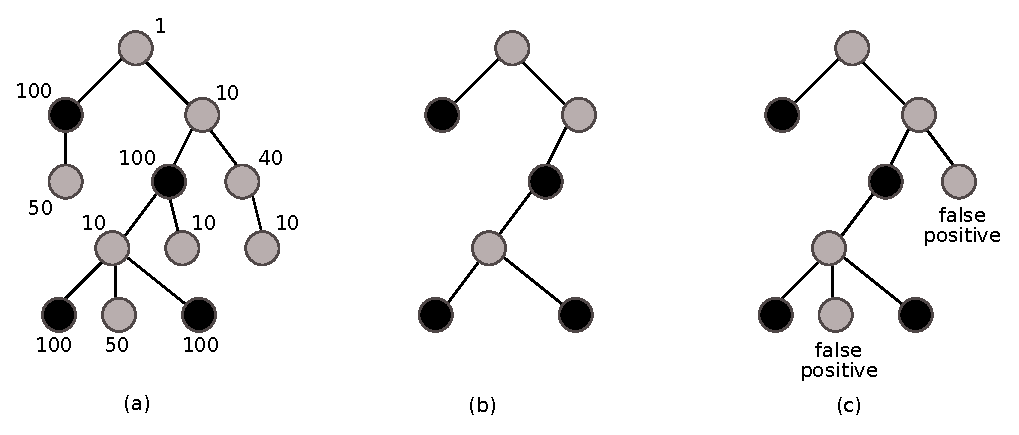
\includegraphics[width=\columnwidth]{hctt.eps}
\caption{(a) CCT; (b) HCCT; and (c) $(\phi,\varepsilon)$-HCCT. Hot nodes are darker. The number close to each node is the frequency count of the corresponding calling context. In this example $N=581$, $\phi=1/10$, and $\varepsilon=1/30$: the approximate HCCT includes all contexts with frequency $\ge\lfloor\phi N\rfloor=58$  and no context with frequency $\le\lfloor(\phi-\varepsilon) N\rfloor=38$.}
\label{fig:HCCT}
\end{figure} 


%------------------------------------------
\subsection{Approach}
\label{ss:approach}

Let $N$ be the number of calling contexts encountered during a program's execution: $N$ equals the number of nodes of the call tree, the sum of the frequency counts of CCT nodes, as well as the number routine invocations in the execution trace. Given a frequency threshold $\phi\in[0,1]$, we will regard a calling context as {\em hot} if the frequency count of the corresponding CCT node is larger than $\lfloor\phi N\rfloor$. All the other contexts are considered {\em cold}. We define the {\em Hot Calling Context Tree (HCCT)} as the (unique) subtree of the CCT obtained by pruning all cold nodes that are not ancestors of a hot node. In graph theory, the HCCT corresponds to the Steiner tree of the CCT with hot nodes used as terminals, i.e., to the minimal connected subtree of the CCT spanning hot nodes. An example of HCCT is given in Figure~\ref{fig:HCCT}(b). It is worth noticing that all hot nodes are included in the HCCT and that all its leaves are necessarily hot (the converse, however, is not true).

The HCCT is the most compact data structure representing information about hot calling contexts. The space lower bound for the heavy hitters problem (see Section~\ref{ss:frequent}) extends to the problem of computing the HCCT, that cannot be calculated exactly in small space (in particular, using a space asymptotically smaller than the entire CCT). Hence, we relax the problem and compute an {\em Approximate Hot Calling Context Tree}, which we denote by {\em $(\phi,\varepsilon)$-HCCT}, where $\varepsilon<\phi$ controls the degree of approximation. The $(\phi,\varepsilon)$-HCCT contains all hot nodes (true positives), but may possibly contain some cold nodes without hot descendants (false positives). The true frequency of these false positives, however, is guaranteed to be at least $\lfloor(\phi-\varepsilon) N\rfloor$. Similarly to the HCCT, the $(\phi,\varepsilon)$-HCCT can be thought of as a minimal subtree of the CCT spanning a set of $(\phi,\varepsilon)$-heavy hitters. Differently from the HCCT, a $(\phi,\varepsilon)$-HCCT is not uniquely defined, since the set of $(\phi,\varepsilon)$-heavy hitters is not unique: in particular, nodes with frequencies smaller than $\lfloor\phi N\rfloor$ and larger than $\lfloor(\phi-\varepsilon) N\rfloor$ may be either included in such a set or not.

The Venn diagram in Figure~\ref{fig:venn} summarizes some important relations:

\begin{itemize}

\item H$\,\subseteq\,$A, where H is the set of hot contexts and A is a set of $(\phi,\varepsilon)$-heavy hitters. Nodes in A$\,\setminus\,$H are false positives.

\item H$\,\subseteq\,$HCCT. Nodes in HCCT$\,\setminus\,$H are cold nodes that have a descendant in H.

\item A$\,\subseteq$$(\phi,\varepsilon)$-HCCT. Nodes in $(\phi,\varepsilon)$-HCCT$\,\setminus\,$A are cold nodes that have a descendant in A.

\item HCCT$\,\subseteq$$(\phi,\varepsilon)$-HCCT, as implied by the previous inclusions. Both of them are connected subtrees of the full CCT.

\end{itemize}

\begin{figure}[t]
\center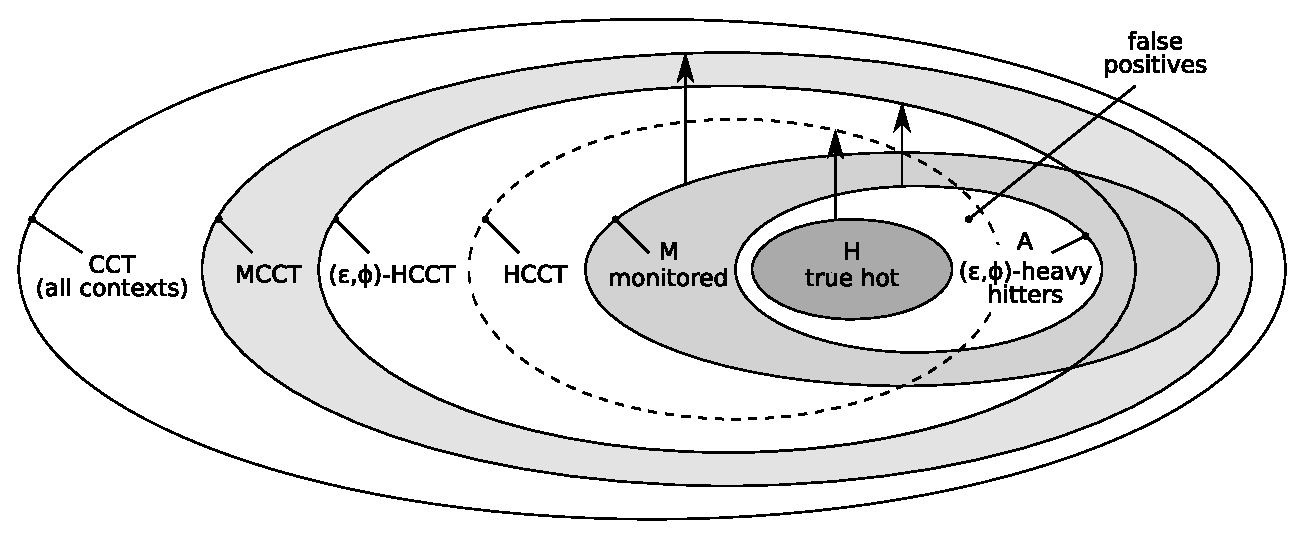
\includegraphics[width=\columnwidth]{venn.eps}
\caption{Tree data structures and calling contexts classification. We use graphical notation S $\uparrow$ T to indicate that T is the minimal subtree of the CCT spanning all nodes in S.}
\label{fig:venn}
\end{figure} 

\noindent Figure~\ref{fig:venn} also introduces two additional sets: the set M of monitored nodes and the subtree MCCT spanning all nodes in M. To compute the set A of $(\phi,\varepsilon)$-heavy hitters, we use as subroutines counter-based streaming algorithms that monitor a slightly larger set M$\,\supseteq\,$A. When a user query asks for the most frequent contexts, these algorithms prune M and return A. In addition to M, our algorithm maintains the subtree MCCT of the CCT consisting of the nodes in M and of all their ancestors. At query time, the MCCT is appropriately pruned and the $(\phi,\varepsilon)$-HCCT$\,\subseteq\,$MCCT is returned. 

\paragraph{Discussion and Example.} To understand why the heavy hitters and the approximate HCCT are not maintained directly, but derived by pruning M and MCCT, respectively, consider the following example: the execution trace contains the initial invocation of the {\tt main} function, which in turn invokes once a routine $p$ and $N-2$ times a different routine $q$. Assume that $N\ge 8$, $\varepsilon=1/4$, $\phi=1/2$, and that the counter-based streaming subroutine can maintain at least three counters. Then only node $q$ has frequency larger than $\lfloor(\phi-\varepsilon)N\rfloor$ and is a $(\phi,\varepsilon)$-heavy hitter, but the algorithm will maintain in M both $p$ and $q$ together with their exact frequencies. Since $p$ has frequency 1, it would be an error returning it as a heavy hitter. For this reason, M needs to be post-processed in order to eliminate low-frequency items that may be included when there are more available counters than heavy hitters. Details on updating and querying M and MCCT are given in Section~\ref{ss:update}.


%------------------------------------------
\subsection{Data Structures Update and Query}
\label{ss:update}

At each function call, the set M of monitored contexts is updated by a counter-based streaming algorithm (see Section~\ref{ss:frequent}). When M is changed, the subtree MCCT spanning nodes in M needs to be brought up to date as well. To describe how this happens, we assume that the interface of the streaming algorithm provides two main functions:

\begin{description}

 \item {\tt update(x,M)}$\rightarrow\,${\tt V}: given a calling context $x$, update M to reflect the new occurrence of $x$ in the stream (e.g., if $x$ was already monitored in M, its frequency count may be increased by one). The {\tt update} function might return a set V of {\em victim} contexts that were previously monitored in M and are evicted during the update (as a special case, $x$ itself may be considered as a victim if the algorithm decides not to monitor it).

\item {\tt query(M)}$\rightarrow\,${\tt A}: remove low-frequency items from M and return the subset A of $(\phi,\varepsilon)$-heavy hitters (see Figure~\ref{fig:venn}).
\end{description}

\noindent Details on the implementation of {\tt update} and {\tt query} depend on the specific streaming algorithm. 

Similarly to the CCT, during the construction of the MCCT we maintain a cursor pointer that points to the current calling context, creating a new node if the current context $x$ is encountered for the first time (see Section~\ref{ss:callingContextTree}). Additionally, we prune the MCCT according to the victim contexts returned by the streaming {\tt update} operation (these contexts are no longer monitored in M). The pseudocode of the pruning algorithm is given in Figure~\ref{fig:update}. Since the tree must remain connected, victims can be removed from the MCCT only if they are leaves. Moreover, removing a victim might expose a path of unmonitored ancestors that no longer have descendants in M: these nodes are pruned as well. The current context $x$ is never removed from the MCCT, even if it is not necessarily monitored in M. This guarantees that no node in the path from the tree root to $x$ will be removed: these nodes have at least $x$ as a descendant and the leaf test (line 3 in Figure~\ref{fig:update}) will always fail.


\begin{figure}[t]
\begin{frameprog}{\columnwidth}{}
{\tt prune}$($x, MCCT$)$: \\
\N \> $V$ $\gets$ {\tt update}(x, M) \\
\N \>  \FOREACH\ context $v\in V\,\backslash \{x\}$ \\
\N \> \> \WHILE\ ($v$ is a leaf in MCCT $\wedge$ $v\not\in$ M) \DO \\
\N \> \> \> remove $v$ from MCCT \\
\N \> \> \> $v$ $\gets$ parent$(v)$ \\
\end{frameprog}
\caption{On-line pruning algorithm.}
\label{fig:update}
\end{figure} 



A similar pruning strategy can be used to compute the $(\phi,\varepsilon)$-HCCT from the MCCT. The streaming {\tt query} operation is first invoked on M, returning the support A of the $(\phi,\varepsilon)$-HCCT. All MCCT nodes that have no descendant in A are then removed, following bottom up path traversals as in the prune operation.

%------------------------------------------
\subsection{Discussion}
\label{ss:discussion}

Compared to the standard approach of maintaining the entire CCT, our solution requires to store the heavy hitters data structure M and the subtree MCCT spanning nodes in M. The space required by M depends on the specific streaming algorithm that is used as a subroutine, and is roughly proportional to $1/\varepsilon$ (see Section~\ref{ss:frequent} for the exact bounds). This space can be customized by appropriately choosing $\varepsilon$, e.g., according to the amount of available memory. An appropriate choice of $\varepsilon$ appears to be crucial for the effectiveness of our approach: smaller values of $\varepsilon$ guarantee more accurate results (less false positives and more precise counters), but imply a larger memory footprint. As we will see experimentally in Section~\ref{se:results}, the high skewness of context frequency distribution guarantees the existence of very convenient tradeoffs between accuracy and space.

The MCCT consists of nodes corresponding to contexts monitored in M and of all their ancestors, which may be cold contexts without a corresponding entry in M. Hence, the space required by the MCCT  dominates the space required by M. The number of cold ancestors cannot be analyzed theoretically: it depends on properties of the execution trace and on the structure of the calling context tree. In Section~\ref{se:results} we will show that in practice this amount is negligible with respect to the number of entries in M.

Updates of the MCCT can be performed very quickly. As we will see in Section~\ref{se:implementation}, the streaming {\tt update} operation requires constant time. Moreover, our implementation hinges upon very simple and cache-efficient data structures, with no need for time-consuming hashing. Simple amortized analysis arguments also show that the amortized running time of tree pruning is constant. 

Differently from previous approaches such as, e.g., adaptive bursting~\cite{ZSCC06}, the MCCT adapts automatically to the case where the hot calling contexts vary over time, and new calling patterns are not likely to be lost. Contexts that are growing more popular are added to the tree as they become more frequent, while contexts that lose their popularity are gradually replaced by hotter contexts and are finally discarded. This guarantees that heavy hitters queries can be issued at any point in time, and will always be able to return the set of hot contexts up to that time.

Our data-streaming based approach is orthogonal to previous techniques and can be integrated, e.g., with sampled stack-walking~\cite{AS00, W00} or with more recent techniques such as static and adaptive bursting~\cite{ZSCC06}. In addition to frequency counts, it can be extended to support arbitrary performance metrics, exploiting the ability of some streaming algorithms to compute the heavy hitters in weighted item sets. 


%--------------------------------------------------------------------------------
\section{Implementation and Engineering}
\label{se:implementation}

We implemented in C three variants of the HCCT construction algorithm described in Section~\ref{se:hot}, based on three different streaming algorithms for the computation of frequent items: Space Saving~\cite{MAA06}, Sticky Sampling~\cite{MM02}, and Lossy Counting~\cite{MM02}. In our experiments, Sticky Sampling consistently proved itself to be less efficient and accurate than its competitors, so we will not mention it any further. All our implementations (including the construction of the entire CCT) are cast in a common framework in which different streaming algorithms can be plugged in.

We use a first-child, next-sibling representation for calling context trees. Each MCCT node also contains a pointer to its parent, the routine ID, the call site, and the performance metrics. The first-child, next-sibling representation is very space-efficient and still guarantees that the children of each node can be explored in time proportional to their number. According to our experiments with several benchmarks, the average number of scanned children is a small constant around 2-3, so this representation turns out to be convenient also for checking whether a routine ID already appears among the children of a node. The parent field, which is needed to perform tree pruning efficiently (see Figure~\ref{fig:update}), is not required in CCT nodes. As routine ID, we use the routine address. Overall, CCT and MCCT nodes require 20 and 24 bytes, respectively, on 32 bit architectures. Using the bit stealing technique, we also encode in one of the pointer fields a Boolean flag that tells if the calling context associated with the node is monitored in the streaming data structure M, without increasing the number of bytes per node. 

To improve time and space efficiency, we allocate nodes through a custom, page-based allocator, which maintains blocks of fixed size. 
Any additional algorithm-specific information needed to maintain the heavy hitters is stored as trailing fields within fat MCCT nodes.

We now describe our implementation of the streaming algorithms, focusing on Space Saving (SS) and Lossy Counting (LC).
 
%------------------------------------------
\subsection{Space Saving}
\label{ss:ss}

Space Saving~\cite{MAA06} monitors a set of $1/\varepsilon=|M|$ pairs of the form $(item, count)$, initialized by the first $1/\varepsilon$ distinct items and their exact counts. After the init phase, when a calling context $c$ is observed in the stream the {\tt update} operation (see Section~\ref{ss:update}) works as follows: 

\begin{enumerate} 

\item if $c$ is monitored, the corresponding counter is incremented; 

\item if $c$ is not monitored, the $(item, count)$ pair with the smallest count is chosen as a victim and has its item replaced with $c$ and its count incremented. Heavy hitters queries are answered by returning entries in $M$ such that count $\geq \lfloor\phi N\rfloor$.

\end{enumerate}

\noindent The update time is bounded by the dictionary operation of checking whether an item is monitored, and by the priority queue operations of finding and maintaining the item with minimum count. In our setting, we can avoid the dictionary operation using the cursor pointer to the MCCT: using this pointer, we can directly access the {\tt monitored} flag of the MCCT node associated with the current context. The priority queue must support two operations, {\tt find-min} and {\tt increment}, which return the item with minimum count and increment a counter, respectively. In~\cite{MAA06}, it is suggested to use an ordered bucket list, where each bucket points to a list of items (MCCT nodes) with the same count, and buckets are ordered by increasing count values. 

In addition to the implementation realized by the Space Saving authors~\cite{MAA06}, we devised a more efficient variant based on a lazy priority queue. We will refer to our implementation as {\em Lazy Space Saving} (LSS). We use an unordered array M of size $1/\varepsilon$, where each array entry points to an MCCT node. We also (lazily) maintain the value {\tt min} of the minimum counter and the smallest index {\tt min-idx} of an array entry that points to a monitored node with counter equal to {\tt min}. The {\tt increment} operation does not change M, since counters are stored directly inside MCCT nodes. However, {\tt min} and {\tt min-idx} may become temporarily out of date after an {\tt increment}: this is why we call the approach lazy. The {\tt find-min} operation described in Figure~\ref{fig:findMin} restores the invariant property on {\tt min} and {\tt min-idx}: it finds the next index in M with counter equal to {\tt min}. If such an index does not exist, it completely rescans M in order to find a new {\tt min} value and its corresponding {\tt min-idx}.

\begin{figure}[t]
\begin{frameprog}{\columnwidth}{}
{\tt find-min}$()$: \\
\N \> \WHILE\ $( M[$min-idx$] \neq$ min $\wedge$ min-idx $\leq M )$ \DO \\
\N \> \> min-idx $\gets$ min-idx $+ 1$ \\
\N \> \IF\ $($min-idx $> M)$ \THEN \\
\N \> \> min $\gets$ minimum in $M$ \\
\N \> \> min-idx $\gets$ smallest index $j$ such that $M[j] =$ min \\
\N \> \RETURN\ min \\
\end{frameprog}
\caption{{\tt find-min} operation used in Lazy Space Saving.}
\label{fig:findMin}
\end{figure} 

\begin{lemma}
After a {\tt find-min} query, the lazy priority queue correctly returns the minimum counter value in O(1) amortized time.
\end{lemma}
\begin{proof}
Counters are never decremented. Hence, at any time, if a monitored item with counter equal to {\tt min} exists, it must be found in a position larger than or equal to {\tt min-idx}. This yields correctness.

To analyze the running time, let $\Delta$ be the value of {\tt min} after $k$ {\tt find-min} and {\tt increment} operations. Since there are $|M|$ counters $\ge\Delta$, counters are initialized to $0$, and each {\tt increment} operation adds 1 to the value of a single counter, it must be $k\ge |M|\Delta$. For each distinct value assumed by {\tt min}, the array is scanned twice. We therefore have at most $2\Delta$ array scans each of length $|M|$, and the total cost of {\tt find-min} operations throughout the whole sequence of operations is upper bounded by $2|M|\Delta$. It follows that the amortized cost is $(2|M|\Delta)/k\leq 2$.
\end{proof}


%------------------------------------------
\subsection{Lossy Counting}
\label{ss:lc}

Lossy Counting~\cite{MM02} maintains a set M of triples of the form (item, count, $\Delta$), where count represents the exact frequency of the item since it was last inserted in M and $\Delta$ is the maximum possible underestimation of count: the algorithm guarantees that at any time the true frequency of a monitored item is $\leq\,$count$\,+\,\Delta$. The incoming stream is conceptually divided into bursts of width $\lceil 1/\varepsilon\rceil$.  During burst $i$, if an item $x$ arrives that already exists in M, the corresponding count is incremented. Otherwise:

\begin{itemize}
\item if $x$ corresponds to a node $v$ with count $c$ that is an ancestor of another node in M, we increment $c$ by 1, leave $\Delta$ untouched, and then add $(x, c, \Delta)$ to M;
\item otherwise, we add $(x, 1, i-1)$ to M.
\end{itemize}

\noindent We slightly modified the insertion algorithm of~\cite{MM02} to achieve better precision by exploiting the advantages of the MCCT data structure.

At the end of burst $i$, M is pruned by deleting entries such that $($count$\,+\,\Delta)\leq i$: the set $V$ of victims returned by the {\tt update} operation (see Section~\ref{ss:update}) is therefore always empty, except at burst boundaries. Heavy hitters queries are answered by returning entries in M such that count$\,+\,\Delta\geq \lfloor\phi N\rfloor$; again, we modified the original algorithm to reduce -- sometimes considerably -- the number of false positives returned in the answer.

Since triples are dynamically added to and deleted from M, it is convenient to maintain M using an unordered linked list. For the sake of efficiency, in our implementation we superimpose M on the MCCT by allocating fat MCCT nodes containing $\Delta$ and the pointer to the next element of M in addition to the standard fields. Hence, Lossy Counting uses 28 bytes per node. Checking whether an item is monitored can be done quickly as described in Section~\ref{ss:ss}. Every $\lceil 1/\varepsilon\rceil$ operations M is scanned and removed items are marked {\tt unmonitored} and pruned from the MCCT as described in Figure~\ref{fig:update}.

%--------------------------------------------------------------------------------
\section{Experimental Evaluation}
\label{se:results}

In this section, we present an extensive experimental study of our data-streaming based profiling mechanism. We implemented several variants of space-efficient context-sensitive profilers and we analyzed their performances and the accuracy of the produced $(\phi,\varepsilon)$-HCCT with respect to several metrics and using many different parameter settings. Our test suite includes profilers based on the three different streaming algorithms discussed in Section~\ref{se:implementation}: Lazy Space Saving (LSS), Bucket Space Saving (BSS), and Lossy Counting (LC). Besides the exahustive approach, where each routine call and return is instrumented, we integrate our implementations with previous techniques aimed at reducing time overhead: we focus in particular on static bursting and adaptive bursting with re-enablement~\cite{ZSCC06}, which offer very convenient time-accuracy tradeoffs. The experimental analysis not only confirms, but reinforces the theoretical prediction: the $(\phi,\varepsilon)$-HCCT represents the hot portions of the full CCT very well using only an extremely small percentage of the space required by the entire CCT: all the hottest calling contexts are always identified correctly, their counters are very accurate, and the number of false positives is rather small. Using the bursting technique, the running time overhead can be kept under control without affecting accuracy in a substantial way. Before discussing the results, we present the details of our experimental methodology, focusing on benchmarks and accuracy metrics, and we describe how the parameters of the streaming algorithms can be tuned. 

%------------------------------------------
\subsection{Methodology and Experimental Setup}
\label{ss:methodology}

\paragraph{Benchmarks.}  Tests were performed on a variety of large-scale Linux applications, including graphics programs ({\tt inkscape} and {\tt gimp}), an hexadecimal file viewer ({\tt ghex2}), audio players/editors ({\tt amarok} and {\tt audacity}), an archiver ({\tt ark}), an Internet browser ({\tt firefox}), an HTML editor ({\tt quanta}), a chat program ({\tt pidgin}), the Open Office suite for word processing ({\tt oowriter}), spreadsheets ({\tt oocalc}), and drawing ({\tt ooimpress}). To ensure deterministic replay of the execution of the interactive applications in out test suite, we used the PIN dynamic instrumentation framework~\cite{Pin05} to record timestamped execution traces for typical usage sessions. After the startup, in each session we interactively used the application for approximately ten up to twenty minutes: e.g., we created a $420\times 300$ pixel image with {\tt gimp} applying a variety of graphic filters and color effects, we reproduced fifty images in slideshow mode with {\tt gwenview}, we played a ten minutes audio file with {\tt amarok}, and we wrote a two pages formatted text, including tables, with {\tt oowriter}. Statistical information about test sets is shown in Table~\ref{tab:CCTsize}: even short sessions of a few minutes result in CCTs consisting of tens of millions of calling contexts, whereas the call graph has only a few thousands nodes. The number of distinct call sites is roughly one order of magnitude larger than the call graph. 

\paragraph{Metrics.} We test the accuracy of the $(\phi,\varepsilon)$-HCCT produced by our profilers according to a variety of metrics:

\begin{enumerate}

\item Degree of overlap, considered in~\cite{AR01, AS00, ZSCC06}, is used to measure the completeness of the $(\phi,\varepsilon)$-HCCT with respect to the full CCT and defined as follows:
$$overlap((\phi,\varepsilon){\mbox{-HCCT,CCT}})=\frac{1}{N}\sum_{\mbox{\footnotesize{arcs}}~e\in (\phi,\varepsilon)\mbox{\footnotesize{-HCCT}}}w(e)$$
where $N$ is the total number of routine activations (corresponding to the CCT total weight) and $w(e)$ is the true frequency of the target node of arc $e$ in the CCT.

\item Hot edge coverage, introduced in~\cite{ZSCC06}, measures the percentage of hot edges of the CCT that are covered by the $(\phi,\varepsilon)$-HCCT, using an edge-weight threshold $\tau\in [0,1]$ to determine hotness. Since $(\phi,\varepsilon)$-HCCT$\subseteq$CCT, hot edge coverage can be defined as follows:
\begin{small}
$$\hspace{-0mm}cover((\phi,\varepsilon){\mbox{-HCCT,CCT}},\tau)=\frac{|\{e\in(\phi,\varepsilon){\mbox{-HCCT:}}\,w(e)\ge\tau H\}|}{|\{e\in\mbox{CCT:}\,w(e)\ge\tau H\}|}$$
\end{small}
where $H$ is the weight of the hottest CCT arc.

\item Maximum frequency of uncovered calling contexts, where a context is uncovered if is not included in the $(\phi,\varepsilon)$-HCCT:
\begin{small}
$$maxUncov((\phi,\varepsilon){\mbox{-HCCT,CCT}})=\max_{e\in\mbox{CCT}\setminus(\phi,\varepsilon){\mbox{-HCCT}}}\frac{w(e)}{H_1}\times 100$$
\end{small}
Average frequency of uncovered contexts is defined similarly.

\item Number of false positives, i.e., $|A\setminus H|$: the smaller this number, the better the $(\phi,\varepsilon){\mbox{-HCCT}}$ approximates the exact HCCT obtained from CCT pruning.

\item Counter accuracy, i.e., maximum error in the frequency counters of $(\phi,\varepsilon)$-HCCT nodes with respect to their true value in the full CCT:
\begin{small}
$$maxError((\phi,\varepsilon){\mbox{-HCCT}})=\max_{e\in(\phi,\varepsilon){\mbox{-HCCT}}}\frac{|w(e)-\widetilde{w}(e)|}{w(e)}\times 100$$
\end{small}
where $w(e)$ and $\widetilde{w}(e)$ are the true and the estimated frequency of context $e$, respectively. Average counter error is defined similarly.

\end{enumerate}

\noindent An accurate solution should maximize degree of overlap and hot edge coverage, and minimize the remaining metrics.

\paragraph{Platform.}  Our experiments were performed on a 2.53GHz Intel Core2 Duo T9400 with 128KB of L1 data cache, 6MB of L2 cache, and 4 GB of main memory DDR3 1066, running Ubuntu 8.04, Linux Kernel 2.6.24, 32 bit.

\begin{table}[t]
\caption{Typical thresholds}
\centering
\begin{small}
\begin{tabular}{c c c c}
\hline\hline
  & HCCT nodes  & HCCT nodes & HCCT nodes \\ 
Benchmark & $\phi=10^{-3}$  & $\phi=10^{-5}$ & $\phi=10^{-7}$ \\ 
\hline
audacity & 112 & 9\,181 & 233\,362 \\
dolphin & 97 & 14\,563 & 978\,544 \\
gimp & 96 & 15\,330 & 963\,708 \\
inkscape & 80 & 16\,713 & 830\,191 \\
oocalc & 136 & 13\,414 & 1\,339\,752 \\
quanta & 94 & 13\,881 & 812\,098 \\
\hline
\end{tabular}
\end{small}
\label{tab:phi}
\end{table}


%------------------------------------------
\subsection{Parameter Tuning}
\label{ss:tuning}

Before describing our experimental findings, we discuss how to choose parameters $\phi$ and $\varepsilon$ to be provided as input to the streaming algorithms. According to the theoretical analysis, an accurate choice of $\phi$ and $\varepsilon$  might greatly affect the space used by the algorithms and the accuracy of the solution. In our study we considered many different choices of $\phi$ and $\varepsilon$ across rather heterogeneous sets of benchmarks and execution traces, always obtaining similar results that we summarize below. 

A rule of thumb about $\phi$ and $\varepsilon$ validated by previous experimental studies~\cite{CH08} suggests that it is sufficient to choose $\varepsilon=\phi/10$ in order to obtain high counter accuracy and a small number of false positives. We found this choice overly pessimistic in our scenario: the extremely skewed cumulative distribution of calling context frequencies shown in Figure~\ref{fig:skewness} makes it possible to use much larger values of $\varepsilon$ without sacrificing accuracy. This yields substantial benefits on the space usage, which is roughly proportional to $1/\varepsilon$. Unless otherwise stated, in all our experiments we used $\varepsilon=\phi/5$.

Let us now consider the choice of $\phi$: $\phi$ is the hotness threshold with respect to the stream length $N$, i.e., to the number of routine enter events. However, $N$ is unknown {\em a priori} during profiling, and thus choosing $\phi$ appropriately may appear to be difficult: too large values might result in returning very few hot calling contexts (even no context at all in some extreme cases), while too small values might result in using too much space and returning too many contexts without being able to discriminate accurately which of them are actually hot. Our experiments suggest that an appropriate choice of $\phi$ is mostly independent of the specific benchmark and of the stream length: as shown in Table~\ref{tab:phi}, different benchmarks have HCCT sizes of the same order of magnitude when using the same $\phi$ threshold (results for omitted benchmarks are similar). This is a consequence of the skewness of context frequency distribution, and greatly simplifies the choice of $\phi$ in practice. Unless otherwise stated, in  our experiments we used $\phi=10^{-4}$, which corresponds to mining roughly the hottest 1\,000 calling contexts.

%------------------------------------------
\subsection{Accuracy: exact HCCT}
\label{ss:accuracy-hcct}

We first discuss the accuracy of the exact HCCT with respect to the full CCT. Since the HCCT is a subtree of the $(\phi,\varepsilon)$-HCCT computed by our algorithms, the results described in this section apply to the $(\phi,\varepsilon)$-HCCT, as well. In particular, the values of degree of overlap and hot edge coverage on the HCCT are a lower bound to the corresponding values in the  $(\phi,\varepsilon)$-HCCT, while the frequency of uncovered contexts is an upper bound.

\begin{figure}[t]
\center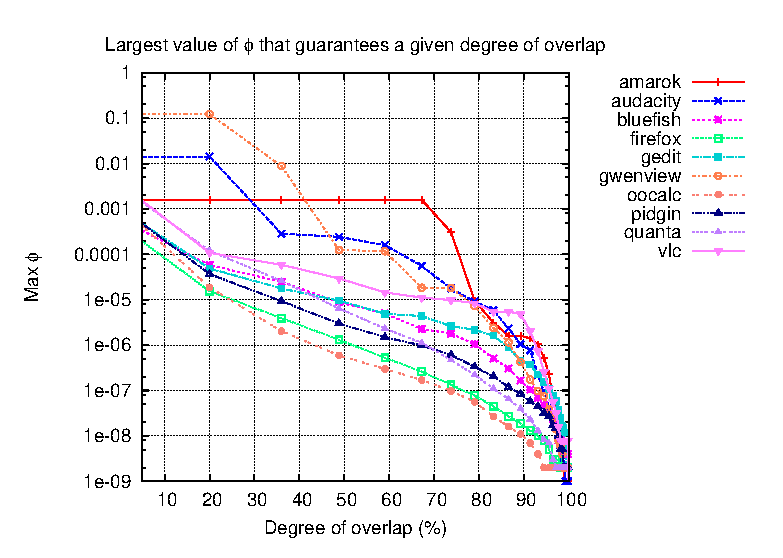
\includegraphics[width=\columnwidth]{charts/maxphi.eps}
\caption{Relation between $\phi$ and degree of overlap between the exact HCCT and the full CCT on a representative subset of benchmarks.}
\label{fig:degreeOfOverlap}
\end{figure}

\begin{figure}[t]
\center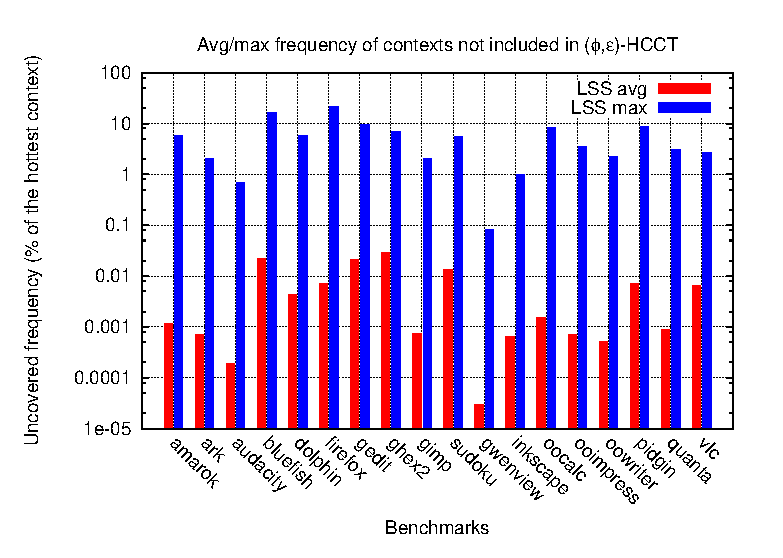
\includegraphics[width=\columnwidth]{charts/avg-max-uncovered.eps}
\caption{Maximum and average frequency of calling contexts not included in the $(\phi,\varepsilon)$-HCCT generated by LSS. Results for LC are almost identical and are not shown in the chart.}
\label{fig:frequencyUncovered}
\end{figure} 

\begin{figure}[t]
\center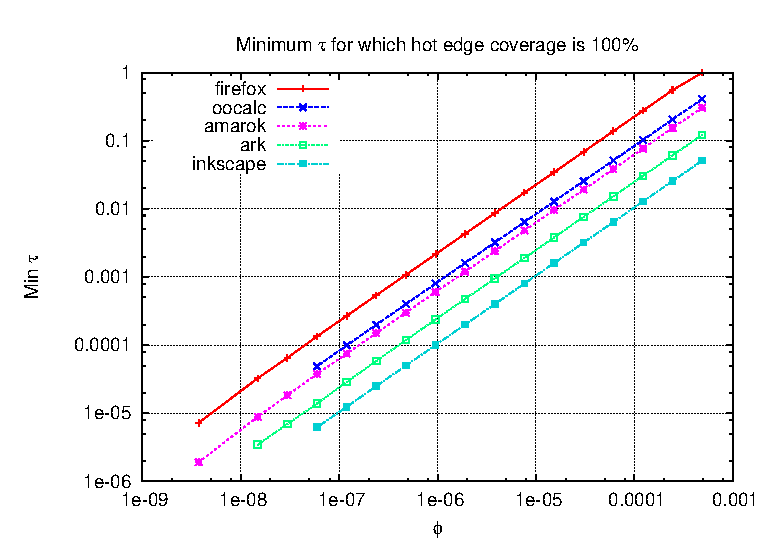
\includegraphics[width=\columnwidth]{charts/mintau.eps}
\caption{Hot edge coverage of the exact HCCT: relation between $\phi$ and edge-weight threshold $\tau$.}
\label{fig:hotEdgeCoverage}
\end{figure} 

It is not difficult to see that the cumulative distribution  of calling context frequencies shown in Figure~\ref{fig:skewness} corresponds exactly to the degree of overlap with the full CCT. This distribution roughly satisfies the $10\%\,$-$\,90\%$ rule: hence, with only $10\%$ of hot contexts, we have a degree of overlap around $90\%$ on all benchmarks. Figure~\ref{fig:degreeOfOverlap} illustrates the relationship between degree of overlap and hotness threshold, plotting the value $\widetilde\phi$ of the largest hotness threshold  for which a given degree of overlap $d$ can be achieved: using any $\phi\leq\widetilde\phi$, the achieved degree of overlap will be larger than or equal to $d$. The value of $\widetilde\phi$ decreases as $d$ increases: if we want to achieve a larger degree of overlap, we must include in the HCCT a larger number of nodes, which corresponds to choosing a smaller hotness threshold. However, when computing the $(\phi,\varepsilon)$-HCCT, the value of $\phi$ indirectly affects the space used by the algorithm and in practice cannot be too small (see Section~\ref{ss:tuning}). By analyzing hot edge coverage and uncovered frequency, we will show below that even when the degree of overlap is not particularly large, the HCCT and the $(\phi,\varepsilon)$-HCCT are nevertheless good approximations of the full CCT: values of $\phi\in[10^{-4},10^{-6}]$ represent on all our benchmarks a good tradeoff between accuracy and space reduction.

Consider, as an example, $\phi=10^{-4}$, which yields degree of overlap as small as $10\%$ on two of the less skewed benchmarks ({\tt oocalc} and {\tt firefox}). In this apparently bad scenario, Figure~\ref{fig:frequencyUncovered} analyzes how the remaining $90\%$ of the total CCT weight is distributed among uncovered contexts: the average frequency of uncovered contexts is about $0.01\%$ of the frequency of the hottest context, and the maximum frequency is typically less than $10\%$. This suggests that uncovered contexts are likely to be uninteresting with respect to the hottest contexts, and that the distribution of calling context frequencies obeys a ``long-tail, heavy-tail'' phenomenon: the CCT contains a huge number of calling contexts that rarely get executed, but overall these low-frequency contexts account for a significant fraction of the total CCT weight. 

Figure~\ref{fig:hotEdgeCoverage} confirms this intuition, showing that the HCCT represents the hot portions of the full CCT remarkably well even for values of $\phi$ for which the degree of overlap may be small. The figure plots, as a function of $\phi$, the smallest value $\widetilde\tau$ of the hotness threshold $\tau$ for which hot edge coverage of the HCCT is $100\%$. Results are shown only on some of the less skewed, and thus more difficult, benchmarks. Note that $\widetilde\tau$ is directly proportional to and  roughly one order of magnitude larger than $\phi$. This is because the HCCT contains all contexts with frequency $\ge\lfloor\phi N\rfloor$, and always contains the hottest context (which implies $H_1=H_2$ in the definition of hot edge coverage in Section~\ref{ss:methodology}). Hence, the hot edge coverage is $100\%$ as long as $\lfloor\phi N\rfloor\ge\tau H_1$, which yields $\widetilde\tau=\lfloor\phi N\rfloor/H_1$. The experiment shows that $100\%$ hot edge coverage is always obtained for $\tau\ge 0.01$. As a frame of comparison, notice that the $\tau$ thresholds used in~\cite{ZSCC06} to analyze hot edge coverage are always larger than $0.05$, and for those values we always guarantee total coverage.
 
%------------------------------------------
\subsection{Accuracy: $(\phi,\varepsilon)$-HCCT}
\label{ss:accuracy-approx-hcct}

We now discuss the accuracy of the $(\phi,\varepsilon)$-HCCT computed by our algorithms compared to the exact HCCT.
%
Figure~\ref{fig:falsePositives} shows the percentages of cold nodes, true hots, and false positives in the $(\phi,\varepsilon)$-HCCT using $\phi=10^{-4}$ and $\varepsilon=\phi/5$. Both algorithms include in the tree only very few false positives (less than $10\%$ of the total number of tree nodes in the worst case), and Lazy Space Saving consistently proved to be better than Lossy Counting. Figure~\ref{fig:falsePositivesEpsilon} also shows that the number of false positives decreases considerably as we decrease $\varepsilon$, getting very close to $0\%$ on most benchmarks when the ratio $\phi/\varepsilon$ is larger than 10. 

A very interesting feature of our approach is that counter estimates are  very close to the true frequencies, as shown in Figure~\ref{fig:counterAccuracy}. Lossy Counting on average achieves almost exact counters  for the hot contexts ($0.057\%$ average difference from the true frequency), and even the maximum error in the worst case is smaller than $8\%$. Lazy Space Saving as described in this paper computes less accurate counters. The error, however, can be considerably reduced and made comparable to Lossy Counting by maintaining, for each monitored context, the maximum possible overestimation resulting from the initialization of the  counter when the context was last inserted in the data structure~\cite{MAA06}. Due to the lack of space, we defer the details of this improvement to the full version of this paper.

\begin{figure}[t]
\center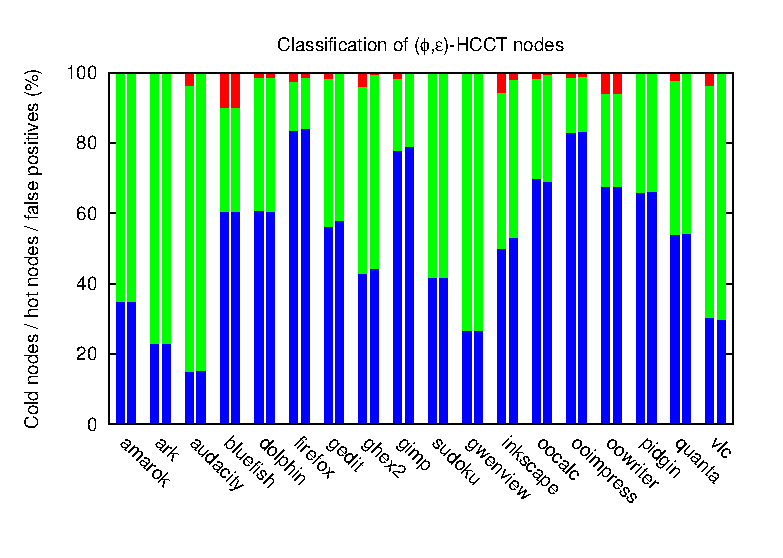
\includegraphics[width=\columnwidth]{charts/false-positives.eps}
\caption{Partition of $(\phi,\varepsilon)$-HCCT nodes into: cold (bottom bar), hot (middle bar), and false positives (top bar) for LSS and LC. The two bars for each benchmark are related to LC (left) and LSS (right), respectively.}
\label{fig:falsePositives}
\end{figure} 

\begin{figure}[t]
\center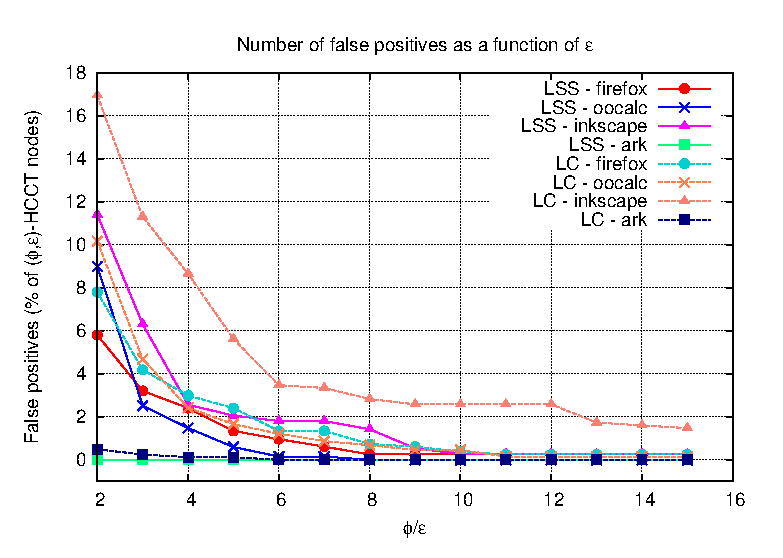
\includegraphics[width=\columnwidth]{charts/false-positives-epsilon.eps}
\caption{False positives in the  $(\phi,\varepsilon)$-HCCT as a function of $\varepsilon$ on a representative subset of benchmarks. The value of $\phi$ is fixed to $10^{-4}$.}
\label{fig:falsePositivesEpsilon}
\end{figure} 

\begin{figure*}[t]
\center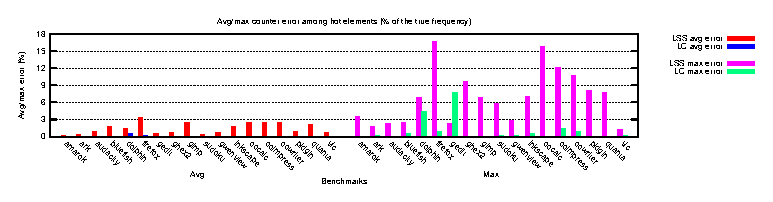
\includegraphics[width=\textwidth]{charts/counter-error.eps}
\caption{Accuracy of context frequencies computed by LSS and LC, measured on hot contexts included in the $(\phi,\varepsilon)$-HCCT.}
\label{fig:counterAccuracy}
\end{figure*} 

\begin{figure*}[t]
\center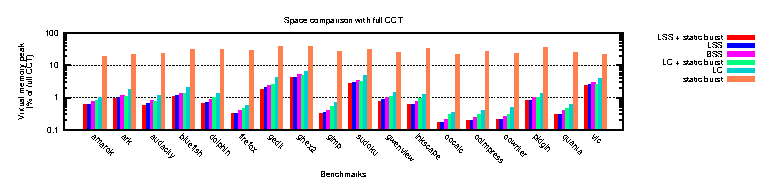
\includegraphics[width=\textwidth]{charts/space.eps}
\caption{Space analysis on several benchmarks of LSS/LC, static and adaptive bursting~\cite{ZSCC06}, and LSS/LC combined with static and adaptive bursting with sampling interval 2 msec, and burst length 0.2 msec.}
\label{fig:VMPeak}
\end{figure*} 


%------------------------------------------
\subsection{Performance}
\label{ss:performance}

To analyze time and space performances of our profilers we consider LSS, LC, BSS (omitted from the previous discussions as it computes exactly the same $(\phi,\varepsilon)$-HCCT as LSS), and the combination of these algorithms with static and adaptive bursting.

\paragraph{Memory Usage.} We first evaluate how much space can be saved by our approach. Figure~\ref{fig:VMPeak} plots the peak memory usage of our profilers as a percentage of the full CCT. We recall that during the computation we store the minimal subtree MCCT of the CCT spanning all monitored contexts. This subtree is eventually pruned to obtain the $(\phi,\varepsilon)$-HCCT (see Section~\ref{ss:approach}). The peak memory usage is proportional to the number of MCCT nodes, which is typically much larger than the actual number of hot contexts obtained after pruning. 
In spite of this, a considerable amount of space is saved by all algorithms. On many benchmarks, our profilers use less than $1\%$ of the space required by the full CCT, and even in the worst case the space usage is about $6.5\%$. Space Saving is always more efficient than Lossy Counting, and the lazy approach is preferable to the bucket-based implementation. It should be noted, however, that the space used in practice by Lossy Counting is much smaller than the theoretical prediction. Quite surprisingly, static bursting also improves space usage (results for adaptive bursting are similar and are not reported in the chart). This depends on the fact that sampling reduces the variance of calling context frequencies: MCCT cold nodes that have a hot descendant are more likely to become hot when sampling is active, and monitoring these nodes reduces the total MCCT size. The histogram also shows that static bursting alone (i.e., without streaming) is not sufficient to reduce the space substantially: in addition to hot contexts, a large fraction of cold contexts is also sampled and included in the CCT. On the {\tt oocalc} benchmark, even adaptive bursting without re-enablement requires 127 times more space than LSS. We also observed that the larger the applications, the larger the space reduction of our approach over bursting alone.

Since the average node degree is a small constant, cold HCCT nodes are typically a fraction of the total number of nodes, as shown in Figure~\ref{fig:falsePositives} for $\phi=10^{-4}$. In our experiments we observed that this fraction strongly depends on the  hotness threshold $\phi$, and in particular decreases with $\phi$: cold nodes that have a hot descendant are indeed more likely to become hot when $\phi$ is smaller.

\paragraph{Time Overhead.} We conclude by analyzing running times. Since our approach is independent of any specific instrumentation mechanisms, and different techniques for tracing routine enter and exit events might incur rather different overheads in practice, we focus on the time required by the analysis routines only, omitting instrumentation times. Compared to the the standard construction of the CCT, streaming algorithms incur a small overhead, which can be considerably reduced by exploiting sampling and bursting techniques: in Figure~\ref{fig:speedup}, we plot the speedup that can be obtained by combining our approach with static bursting and with adaptive bursting. We compared the performance of six variants (from slowest to fastest) for both LSS and LC: full $(\phi,\varepsilon)$-HCCT construction (on the entire routine enter/exit stream), static bursting, adaptive bursting with re-enable ratio equal to $20\%$,  $10\%$,  and $5\%$, and adaptive bursting without re-enablement (for a description of the adaptive bursting technique, we refer the interested reader to~\cite{ZSCC06}). We also considered bursting alone (both static and adaptive), while we omitted sample-driven stack walking, which has been shown to be largely inferior to bursting with respect to the accuracy~\cite{ZSCC06}. The construction of the HCCT greatly benefits from bursting, achieving speedups up to $35\times$. LSS is always faster than LC, but both of them are slower than bursting without streaming: the speedup difference, however, is moderate and for LSS is typically smaller than 2.

As shown in Figure~\ref{fig:sampling-accuracy}, the accuracy of the HCCT (and in particular the hot edge coverage) is not affected substantially by the combination of streaming and bursting (except for adaptive sampling without re-enablement). We take as an example the {\tt vlc} benchmark considered in Figure~\ref{fig:speedup} for $\tau=0.025$: the HCCT computed without bursting has coverage $100\%$, which is also achieved using static busting and adaptive bursting with re-enable ratio $20\%$. The hot edge coverage decreases as sampling becomes more aggressive, but in this experiment is always larger than $78\%$ and $91\%$ for LSS and LC, respectively.


\begin{figure}[t]
\center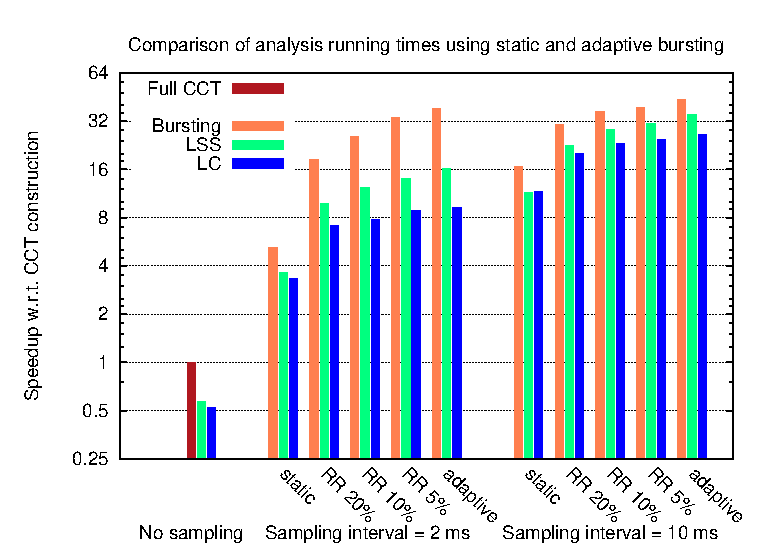
\includegraphics[width=\columnwidth]{charts/speedup.eps}
\caption{Speedup analysis relative to full CCT construction on the {\tt vlc} benchmark for LSS/LC, static and adaptive bursting~\cite{ZSCC06}, and LSS/LC combined with static and adaptive bursting: (1) no sampling (left histogram); (2) sampling interval 2 msec and burst length 0.2 msec (middle histogram); (3) sampling interval 10 msec and burst length 0.2 msec (right histogram). The CCT construction baseline is about 1.5 seconds for $2.5\cdot 10^8$ routine enter/exit events. }
\label{fig:speedup}
\end{figure} 


%--------------------------------------------------------------------------------
\section{Related Work}
\label{se:related}

This section describes research on context sensitive profiling: it focuses on calling context trees and briefly considers other forms of contextual profiling at both inter and intraprocedural level.

\paragraph{Early approaches.} The utility of calling context information was already clear in the 80s: gprof~\cite{GKM82} approximates context sensitive profiles by associating procedure timing with caller-callee pairs rather than with single procedures. This single level of context sensitivity, however, may yield to several inaccuracies~\cite{PF88, S04}. Goldberg and Hall~\cite{HG93}  introduce call path profiles of monotonic program resources and show how they can be computed in Unix processes using interval-based sampling: a call path is a sequence of function pairs in a caller-callee relationship, and the profile is a sorted list of call paths and of their performance metrics. The space usage with this approach can be prohibitive, since at each sample point metrics are recorded along with the entire call stack.

\paragraph{Calling context trees.} Calling context trees have been introduced in~\cite{ABL97} as a practical data structure to associate performance metrics with paths through a program's call graph: Ammons, Ball, and Larus suggest to build a CCT by instrumenting procedure code and to compute metrics by exploiting hardware counters available in modern processors. It has been later observed, however, that exhaustive instrumentation can lead to large slowdown. 

\paragraph{Time-efficiency vs. profile accuracy.} To reduce overhead, Bernat and Miller~\cite{BM04} generate path profiles including only methods of interest, while statistical profilers~\cite{AS00, FMF05, HG93, W00} attribute metrics to calling contexts through periodic sampling of the call stack. For call-intensive programs, sample-driven stack-walking can be orders of magnitude faster than exhaustive instrumentation, but may incur significant loss of accuracy with respect to the complete CCT: sampling guarantees neither high coverage~\cite{BM07} nor accuracy of performance metrics~\cite{ZSCC06}, and its results may be highly inconsistent in different executions. 

\begin{figure}[t]
\center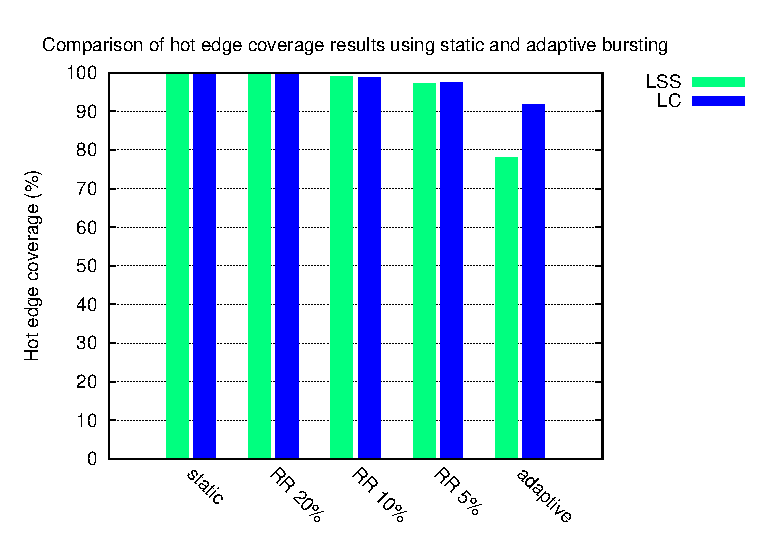
\includegraphics[width=\columnwidth]{charts/sampling-accuracy.eps}
\caption{Hot edge coverage analysis on the {\tt vlc} benchmark for LSS/LC combined with static and adaptive bursting~\cite{ZSCC06} for $\tau=0.025$, with $\phi=4\cdot 10^{-5}$, $\epsilon=\phi/2$, sampling interval 2 msec, and burst length 0.2 msec. Static and adaptive bursting alone always achieve 100\% hot edge coverage in this experiment and are not reported.}
\label{fig:sampling-accuracy}
\end{figure}

A variety of works explores the combination of sampling with bursting~\cite{AR01, HC01, ZSCC06}. Most recently, Zhuang {\em et al.} suggest to perform stack-walking followed by a burst during which the profiler traces every routine call and return~\cite{ZSCC06}: experiments show that adaptive bursting can yield very accurate results. In~\cite{SZ09}, the profiler infrequently collects small call traces that are merged afterwards to build large calling context trees: ambiguities might emerge during this process, and the lack of information about where the partial CCTs should be merged to does not allow it to reconstruct the entire CCT univocally.
The main goal of all these works is to reduce profiling overhead without incurring significant loss of accuracy. 
Our approach is orthogonal to this line of research and regards space efficiency as an additional resource optimization criterion besides profile accuracy and time efficiency. When the purpose of profiling is to identify hot contexts, exhaustive instrumentation, sampling, and bursting might all be combined with our approach and benefit of our space reduction technique.

\paragraph{Reducing space.} A few previous works have addressed techniques to reduce profile data (or at least the amount of data presented to the user) in context sensitive profiling. Incremental call-path profiling lets the user choose a subset of routines to be analyzed~\cite{BM04}. Call path refinement helps users focus the attention on performance bottlenecks by limiting and aggregating the information revealed to the user~\cite{H95}. These works are quite different in spirit from our approach, where only hot contexts are profiled and identified automatically during program's execution. Quite recently, probabilistic calling contexts have been introduced as an extremely compact representation (just a 32-bit value per context), especially useful for tasks such as residual testing, statistical bug isolation, and anomaly-based intrusion detection~\cite{BM07}. Bond and McKinley target applications where coverage of both hot and cold contexts is necessary. This is not the case in performance analysis, where identifying a few hot contexts is typically sufficient to guide code optimization. Hence, although sharing with~\cite{BM07} the common goal of space reduction, our approach targets a rather different application context.

\paragraph{Path profiling.} At the intraprocedural level,  the seminal work of Ball and Larus~\cite{BL96} has spawned much research on flow sensitive profiling~\cite{ABL97, BMS98, L99, AH02, AL04, JBZ04, VNC07, BM05, BM05b}. Ball-Larus path profiling computes a unique number through each possible path in the control flow graph~\cite{BL96}: a path profile determines how many times each acyclic path in a routine executes, extending the more common basic block and edge profiling. Melski and Reps have proposed interprocedural path profiling in order to capture both inter- and intraprocedural control flow~\cite{MR99}. However, their approach does not scale due to the large number of statically possible paths existing across procedure boundaries.

%--------------------------------------------------------------------------------
\section{Conclusions}
\label{se:conclusion}

Calling context trees offer a compact representation of all calling contexts encountered during a program's execution. Even for short runs of medium-sized applications, CCTs can be rather large and difficult to analyze. Motivated by the observation that only a very small fraction of calling contexts are hot, in this paper we have presented a novel technique for improving the space efficiency of the full calling context tree without sacrificing accuracy. By adapting modern data mining techniques, we have devised an algorithm for interprocedural contextual profiling that can discard on the fly cold contexts and appears to be extremely practical. We have evaluated our approach on several large-scale Linux applications, showing significant space saving with respect to the full CCT.

We believe that a careful use of data mining techniques has the potential benefit of enabling some previously impossible dynamic program analysis tasks, which would otherwise be too costly. In particular, our techniques could be applied to certain forms of path profiling: e.g., they could help leverage the scalability problems encountered when collecting performance metrics about interprocedural paths (i.e., acyclic paths that may cross procedure boundaries)~\cite{MR99} or $k$-iteration paths (i.e., intraprocedural cyclic paths spanning up to $k$ loop iterations) for large values of $k$~\cite{SS09}. We plan to investigate these applications in future work.


\acks

We thank the anonymous reviewers for their valuable comments. This work is supported in part by the Italian Ministry for Education,
University, and Research (MIUR) under the PRIN national research project ``AlgoDEEP: Algorithmic challenges for data-intensive processing on emerging computing platforms''.

%--------------------------------------------------------------------------------
\bibliographystyle{abbrvnat}
\softraggedright

\balance
\bibliography{DynamicAnalysis}

\end{document}
